% answers.tex —— 2020 年·全国Ⅰ卷·理科 · 参考答案与详细解析片段
% 由 tools/generate_projects.py 依来源总账自 2020/2020_数学真题_理_试题.md + 2020/2020_数学真题_理_解析正文.md + 2020/2020_数学真题_理_答案要点.md 生成，勿手改（改源 MD 后重跑）


\begin{gknotice}
\textbf{解析归属}：本文档全部解析由本库编写者根据试题独立推导，\textbf{非官方标准答案}。若与官方发布版本不一致，以官方为准。

\textbf{ 卷种提示}：本卷为文理分科时代的旧结构（12 单选 + 4 填空 + 5 必做解答 + 选做题）。\textbf{第 22、23 题的选做内容在现行新课标中已取消}，仅作历史资料保留。其余题目知识点仍在考纲内。
\end{gknotice}

\par\medskip

\gkpart{一、选择题（每小题 5 分，共 60 分）}

\begin{answer}
\gksolhead{1}{}

\textbf{题目}：

若 $z=1+\mathrm i$，则 $\left|z^{2}-2z\right|=$\mbox{（　　）}

\begin{gkopts}(4)
\task A．$0$
\task B．$1$
\task C．$\sqrt2$
\task D．$2$
\end{gkopts}

\Needspace{4\baselineskip}
\textbf{解析}

\Needspace{5\baselineskip}
\textbf{方法一（直接展开）}
\nopagebreak[4]
\[z^{2}=(1+\mathrm i)^{2}=1+2\mathrm i+\mathrm i^{2}=2\mathrm i\]
\nopagebreak[4]
\[2z=2+2\mathrm i\]
\nopagebreak[4]
\[z^{2}-2z=2\mathrm i-(2+2\mathrm i)=-2\]
\nopagebreak[4]
\[\left|z^{2}-2z\right|=|-2|=2\]

\Needspace{5\baselineskip}
\textbf{方法二（配方，更快）}
\nopagebreak[4]
\[z^{2}-2z=(z-1)^{2}-1=\mathrm i^{2}-1=-1-1=-2\]

\gkanswer{答案：D（$2$）}

\par\medskip

\end{answer}
\begin{answer}
\gksolhead{2}{}

\textbf{题目}：

设集合 $A=\left\{x\mid x^{2}-4\le0\right\}$，$B=\{x\mid2x+a\le0\}$，且 $A\cap B=\{x\mid-2\le x\le1\}$，则 $a=$\mbox{（　　）}

\begin{gkopts}(4)
\task A．$-4$
\task B．$-2$
\task C．$2$
\task D．$4$
\end{gkopts}

\Needspace{4\baselineskip}
\textbf{解析}

\Needspace{5\baselineskip}
\textbf{第一步，化简两个集合。}
\nopagebreak[4]
\[x^{2}-4\le0\iff-2\le x\le2\ \Longrightarrow\ A=[-2,\ 2]\]
\nopagebreak[4]
\[2x+a\le0\iff x\le-\frac a2\ \Longrightarrow\ B=\left(-\infty,\ -\frac a2\right]\]

\Needspace{5\baselineskip}
\textbf{第二步，求交集的一般形式。}
\nopagebreak[4]
\[A\cap B=\left[-2,\ \min\left\{2,\ -\frac a2\right\}\right]\]

\textbf{第三步，与已知交集比对。}

\Needspace{5\baselineskip}
已知 $A\cap B=[-2,1]$，右端点为 $1$，而 $1<2$，故右端点由 $-\dfrac a2$ 决定：
\nopagebreak[4]
\[-\frac a2=1\ \Longrightarrow\ a=-2\]

\textbf{验证}：$a=-2$ 时 $B=(-\infty,1]$，$A\cap B=[-2,1]$ 

\gkanswer{答案：B（$-2$）}

\par\medskip

\end{answer}
\begin{answer}
\gksolhead{3}{}

\textbf{题目}：

埃及胡夫金字塔是古代世界建筑奇迹之一，它的形状可视为一个正四棱锥，以该四棱锥的高为边长的正方形面积等于该四棱锥一个侧面三角形的面积，则其侧面三角形底边上的高与底面正方形的边长的比值为\mbox{（　　）}

\begin{gkopts}(2)
\task A．$\dfrac{\sqrt5-1}4$
\task B．$\dfrac{\sqrt5-1}2$
\task C．$\dfrac{\sqrt5+1}4$
\task D．$\dfrac{\sqrt5+1}2$
\end{gkopts}

\Needspace{4\baselineskip}
\textbf{解析}

\gkanswer{第一步，设参数（注意底边设法会影响答案形式）。}

设底面正方形边长为 $2a$，四棱锥的高为 $h$，侧面三角形底边上的高（\textbf{斜高}）为 $m$。

\textbf{第二步，写出几何关系。}

\Needspace{5\baselineskip}
侧面三角形的高 $m$、四棱锥的高 $h$、底面中心到边中点的距离 $a$ 构成直角三角形：
\nopagebreak[4]
\[m^{2}=h^{2}+a^{2}\qquad(\text{i})\]

\textbf{第三步，翻译题目条件。}

\begin{itemize}
\item 以高为边长的正方形面积：$h^{2}$
\item 一个侧面三角形的面积：底为 $2a$、高为 $m$，即 $\dfrac12\times2a\times m=am$
\end{itemize}

\Needspace{5\baselineskip}
条件给出：
\nopagebreak[4]
\[h^{2}=am\qquad(\text{ii})\]

\textbf{第四步，消元求比值。}

\Needspace{5\baselineskip}
把 (ii) 代入 (i)：
\nopagebreak[4]
\[m^{2}=am+a^{2}\]

\Needspace{5\baselineskip}
两边除以 $a^{2}$，令 $t=\dfrac ma$：
\nopagebreak[4]
\[t^{2}-t-1=0\ \Longrightarrow\ t=\frac{1\pm\sqrt5}2\]

\Needspace{5\baselineskip}
取正根：
\nopagebreak[4]
\[\frac ma=\frac{1+\sqrt5}2\]

\textbf{第五步，注意所求的是什么。}

\Needspace{5\baselineskip}
题目问的是"\textbf{侧面三角形底边上的高与底面正方形的边长}的比值"，即
\nopagebreak[4]
\[\frac m{2a}=\frac12\times\frac{1+\sqrt5}2=\frac{\sqrt5+1}4\]

\begin{gktip}
\textbf{易错点}：$\dfrac{\sqrt5+1}2$（选项 D）是著名的\textbf{黄金分割比}，也正是 $\dfrac ma$ 的值。若把底面边长设成 $a$（而不是 $2a$），中途容易搞混"底面边长"与"底面中心到边的距离"，从而错选 D。\textbf{设参数时把边长设成 $2a$ 可以避免出现分数，是好习惯。}
\end{gktip}

\gkanswer{答案：C（$\dfrac{\sqrt5+1}4$）}

\par\medskip

\end{answer}
\begin{answer}
\gksolhead{4}{}

\textbf{题目}：

已知 $A$ 为抛物线 $C:y^{2}=2px\ (p>0)$ 上一点，点 $A$ 到 $C$ 的焦点的距离为 $12$，到 $y$ 轴的距离为 $9$，则 $p=$\mbox{（　　）}

\begin{gkopts}(4)
\task A．$2$
\task B．$3$
\task C．$6$
\task D．$9$
\end{gkopts}

\Needspace{4\baselineskip}
\textbf{解析}

\textbf{第一步，理解两个距离。}

\begin{itemize}
\item 到 $y$ 轴的距离 = 横坐标的绝对值。因抛物线开口向右，$x_A\ge0$，故 $x_A=9$。
\item 到焦点的距离用\textbf{焦半径公式}：抛物线上任一点到焦点的距离等于它到准线的距离，即
\end{itemize}
\nopagebreak[4]
\[|AF|=x_A+\frac p2\]

\Needspace{5\baselineskip}
\textbf{第二步，列方程。}
\nopagebreak[4]
\[9+\frac p2=12\ \Longrightarrow\ \frac p2=3\ \Longrightarrow\ p=6\]

\begin{gktip}
\textbf{方法总结}：抛物线的一切"距离"问题都优先用\textbf{定义}（到焦点距离 = 到准线距离）转化，几乎不需要两点间距离公式。$y^2=2px$ 的焦半径公式 $|AF|=x_A+\dfrac p2$ 应当熟记。
\end{gktip}

\gkanswer{答案：C（$6$）}

\par\medskip

\end{answer}
\begin{answer}
\gksolhead{5}{}

\textbf{题目}：

某校一个课外学习小组为研究某作物种子的发芽率 $y$ 和温度 $x$（单位：$^\circ\mathrm C$）的关系，在 $20$ 个不同的温度条件下进行种子发芽实验，由实验数据 $\left(x_i,y_i\right)\ (i=1,2,\cdots,20)$ 得到下面的散点图：
\nopagebreak[4]
\begin{center}% 2020 全国Ⅰ卷 理5：发芽率-温度散点图（对数饱和形态，数据点按原图形态示意布点）
\begin{tikzpicture}
\begin{axis}[width=8.8cm, height=5cm, font=\small,
  xlabel={温度$/^{\circ}\mathrm{C}$}, ylabel={发芽率},
  xlabel style={at={(1,0)}, anchor=north west},
  ylabel style={at={(0,1)}, anchor=south, rotate=-90},
  xmin=0, xmax=44, ymin=0, ymax=1.08,
  xtick={0,10,20,30,40},
  ytick={0.2,0.4,0.6,0.8,1.0},
  yticklabels={$20\%$,$40\%$,$60\%$,$80\%$,$100\%$},
  axis lines=left, axis line style={-Stealth}]
  \addplot[only marks, mark=square*, mark size=1.3pt] coordinates {
    (10,0.36) (11.5,0.42) (13,0.50) (14.5,0.55) (16,0.58)
    (17.5,0.62) (19,0.64) (20.5,0.68) (22,0.69) (23.5,0.72)
    (25,0.73) (26.5,0.76) (28,0.76) (29.5,0.79) (31,0.80)
    (33,0.82) (35,0.83) (37,0.86) (39,0.86) (40.5,0.88)};
  \addplot[domain=9:41, samples=80, smooth] {0.35*ln(x)-0.45};
\end{axis}
\end{tikzpicture}
\end{center}
\nopagebreak[4]
由此散点图，在 $10\ ^\circ\mathrm C$ 至 $40\ ^\circ\mathrm C$ 之间，下面四个回归方程类型中最适宜作为发芽率 $y$ 和温度 $x$ 的回归方程类型的是\mbox{（　　）}

\begin{gkopts}(2)
\task A．$y=a+bx$
\task B．$y=a+bx^{2}$
\task C．$y=a+b\mathrm e^{x}$
\task D．$y=a+b\ln x$
\end{gkopts}

\Needspace{4\baselineskip}
\textbf{解析}

\textbf{读图}：散点显示，随着温度从 $10\ ^\circ\mathrm C$ 升到 $40\ ^\circ\mathrm C$，发芽率
\begin{itemize}
\item 在低温段（$10\sim20\ ^\circ\mathrm C$）\textbf{上升很快}
\item 在高温段（$25\sim40\ ^\circ\mathrm C$）\textbf{几乎不再上升，趋于平缓（约 $80\%\sim90\%$）}
\end{itemize}

这是典型的\textbf{增长逐渐放缓、趋于饱和}的形态。

\textbf{逐项分析四个模型的图象形状：}

\begin{center}
\begin{tabular}{cllc}
\toprule
选项 & 模型 & 图象特征 & 是否符合 \\
\midrule
A & $y=a+bx$ & 直线，\textbf{匀速}上升 &  无法体现放缓 \\
B & $y=a+bx^{2}$ & 抛物线，$b>0$ 时\textbf{加速}上升 &  越来越陡 \\
C & $y=a+b\mathrm e^{x}$ & 指数，\textbf{爆炸式}增长 &  更陡 \\
D & $y=a+b\ln x$ & 对数，\textbf{增长逐渐放缓} &  \\
\bottomrule
\end{tabular}
\end{center}

\begin{gktip}
\textbf{判据总结}：
\begin{itemize}
\item 增长\textbf{越来越快} → 二次型（$x^2$）或指数型（$\mathrm e^{x}$）
\item 增长\textbf{越来越慢、趋于饱和} → \textbf{对数型}（$\ln x$）或幂函数（$\sqrt x$）
\item 增长\textbf{匀速} → 线性
\end{itemize}

生物学中的"发芽率、生长率随环境因素变化"几乎都是饱和型，选对数模型是常识性判断。
\end{gktip}

\gkanswer{答案：D（$y=a+b\ln x$）}

\par\medskip

\end{answer}
\begin{answer}
\gksolhead{6}{}

\textbf{题目}：

函数 $f(x)=x^{4}-2x^{3}$ 的图象在点 $(1,f(1))$ 处的切线方程为\mbox{（　　）}

\begin{gkopts}(4)
\task A．$y=-2x-1$
\task B．$y=-2x+1$
\task C．$y=2x-3$
\task D．$y=2x+1$
\end{gkopts}

\Needspace{4\baselineskip}
\textbf{解析}

\Needspace{5\baselineskip}
\textbf{第一步，求切点纵坐标。}
\nopagebreak[4]
\[f(1)=1^{4}-2\times1^{3}=1-2=-1\]

切点为 $(1,-1)$。

\Needspace{5\baselineskip}
\textbf{第二步，求斜率。}
\nopagebreak[4]
\[f'(x)=4x^{3}-6x^{2}\]
\nopagebreak[4]
\[k=f'(1)=4-6=-2\]

\Needspace{5\baselineskip}
\textbf{第三步，点斜式。}
\nopagebreak[4]
\[y-(-1)=-2(x-1)\ \Longrightarrow\ y+1=-2x+2\ \Longrightarrow\ y=-2x+1\]

\begin{gktip}
\textbf{验证习惯}：把切点 $(1,-1)$ 代回所得直线：$-2\times1+1=-1$  吻合。选项 A（$y=-2x-1$）斜率对但截距错，正是漏算 $f(1)$ 的结果。
\end{gktip}

\gkanswer{答案：B（$y=-2x+1$）}

\par\medskip

\end{answer}
\begin{answer}
\gksolhead{7}{}

\textbf{题目}：

设函数 $f(x)=\cos\left(\omega x+\dfrac\pi6\right)$ 在 $[-\pi,\pi]$ 的图象大致如下图，则 $f(x)$ 的最小正周期为\mbox{（　　）}
\nopagebreak[4]
\begin{center}% 2020 全国Ⅰ卷 理7：f(x)=cos(ωx+π/6) 的图象（按答案 T=4π/3，即 ω=3/2 精确绘制）
\begin{tikzpicture}
\begin{axis}[width=8.6cm, height=4.6cm, font=\small,
  axis lines=middle, xlabel={$x$}, ylabel={$y$},
  xmin=-3.6, xmax=3.7, ymin=-1.35, ymax=1.45,
  xtick={-3.14159, -1.39626, 3.14159},
  xticklabels={$-\pi$, $-\frac{4\pi}{9}$, $\pi$},
  ytick=\empty,
  every axis x label/.style={at={(current axis.right of origin)}, anchor=west},
  every axis y label/.style={at={(current axis.above origin)}, anchor=south}]
  \addplot[domain=-3.14159:3.14159, samples=200, thick] {cos(deg(1.5*x + pi/6))};
  \node[below left, font=\small] at (axis cs:0,0) {$O$};
\end{axis}
\end{tikzpicture}
\end{center}
\nopagebreak[4]
\begin{gkopts}(4)
\task A．$\dfrac{10\pi}9$
\task B．$\dfrac{7\pi}6$
\task C．$\dfrac{4\pi}3$
\task D．$\dfrac{3\pi}2$
\end{gkopts}

\Needspace{4\baselineskip}
\textbf{解析}

\textbf{第一步，从图中读取关键信息。}

图中明确标注了 $x=-\dfrac{4\pi}9$，从图象看该处是函数的一个\textbf{零点}（曲线穿过 $x$ 轴）。

\textbf{第二步，代入零点条件。}

\Needspace{5\baselineskip}
$\cos u=0\iff u=\dfrac\pi2+k\pi$，故
\nopagebreak[4]
\[\omega\left(-\frac{4\pi}9\right)+\frac\pi6=\frac\pi2+k\pi\qquad(k\in\mathbb Z)\]

\textbf{第三步，解出 $\omega$。}

\Needspace{5\baselineskip}
两边除以 $\pi$：
\nopagebreak[4]
\[-\frac{4\omega}9+\frac16=\frac12+k\]

\nopagebreak[4]
\[-\frac{4\omega}9=\frac13+k\ \Longrightarrow\ \omega=-\frac94\left(\frac13+k\right)=-\frac34-\frac{9k}4=\frac{-3-9k}4\]

\textbf{第四步，用图象特征筛选 $k$。}

由图象在 $[-\pi,\pi]$ 内大约完成\textbf{一个半周期}（有两个完整的波峰波谷结构），可判断 $\omega>0$ 且不太大。

\begin{itemize}
\item $k=-1$：$\omega=\dfrac{-3+9}4=\dfrac64=\dfrac32$ 
\item $k=-2$：$\omega=\dfrac{-3+18}4=\dfrac{15}4$（周期过小，图象会挤成很多个波，与图不符）
\item $k\ge0$：$\omega<0$，舍去
\end{itemize}

取 $\omega=\dfrac32$。

\Needspace{5\baselineskip}
\textbf{第五步，求周期。}
\nopagebreak[4]
\[T=\frac{2\pi}\omega=\frac{2\pi}{\frac32}=\frac{4\pi}3\]

\Needspace{5\baselineskip}
\textbf{验证}：
\nopagebreak[4]
\[f\left(-\frac{4\pi}9\right)=\cos\left(\frac32\times\left(-\frac{4\pi}9\right)+\frac\pi6\right)=\cos\left(-\frac{2\pi}3+\frac\pi6\right)=\cos\left(-\frac\pi2\right)=0\quad\checkmark\]

\begin{gktip}
\textbf{方法总结}：三角函数"看图求周期"的通法是——\textbf{从图中读出一个特殊点（零点、最值点）的坐标，代入方程解出 $\omega$，再用图象的整体形状（周期个数）筛选 $k$}。切忌只凭"看起来周期约为多少"来估算，必须用图上标注的精确数值。
\end{gktip}

\gkanswer{答案：C（$\dfrac{4\pi}3$）}

\par\medskip

\end{answer}
\begin{answer}
\gksolhead{8}{}

\textbf{题目}：

$\left(x+\dfrac{y^{2}}x\right)(x+y)^{5}$ 的展开式中 $x^{3}y^{3}$ 的系数为\mbox{（　　）}

\begin{gkopts}(4)
\task A．$5$
\task B．$10$
\task C．$15$
\task D．$20$
\end{gkopts}

\Needspace{4\baselineskip}
\textbf{解析}

\Needspace{5\baselineskip}
\textbf{拆成两部分分别处理}：
\nopagebreak[4]
\[\left(x+\frac{y^{2}}x\right)(x+y)^{5}=x\cdot(x+y)^{5}+\frac{y^{2}}x\cdot(x+y)^{5}\]

$(x+y)^{5}$ 的通项为 $C_5^{k}x^{5-k}y^{k}$。

\textbf{第一部分}：$x\cdot C_5^{k}x^{5-k}y^{k}=C_5^{k}x^{6-k}y^{k}$

\Needspace{5\baselineskip}
要得 $x^{3}y^{3}$，需 $k=3$（此时 $x$ 的次数为 $6-3=3$ ）：
\nopagebreak[4]
\[\text{\text{系数}}=C_5^{3}=10\]

\textbf{第二部分}：$\dfrac{y^{2}}x\cdot C_5^{k}x^{5-k}y^{k}=C_5^{k}x^{4-k}y^{k+2}$

\Needspace{5\baselineskip}
要得 $x^{3}y^{3}$，需 $k+2=3$ 即 $k=1$（此时 $x$ 的次数为 $4-1=3$ ）：
\nopagebreak[4]
\[\text{\text{系数}}=C_5^{1}=5\]

\Needspace{5\baselineskip}
\textbf{合计}：
\nopagebreak[4]
\[10+5=15\]

\begin{gktip}
\textbf{方法总结}：形如 $(A+B)(x+y)^{n}$ 求某项系数，\textbf{必须分别考虑 $A$ 和 $B$ 与展开式的配合}，两者需要的 $k$ 通常不同。写出乘以 $A$（或 $B$）之后的通项形式，再令次数匹配，是最不容易出错的做法。
\end{gktip}

\gkanswer{答案：C（$15$）}

\par\medskip

\end{answer}
\begin{answer}
\gksolhead{9}{}

\textbf{题目}：

已知 $\alpha\in(0,\pi)$，且 $3\cos2\alpha-8\cos\alpha=5$，则 $\sin\alpha=$\mbox{（　　）}

\begin{gkopts}(2)
\task A．$\dfrac{\sqrt5}3$
\task B．$\dfrac23$
\task C．$\dfrac13$
\task D．$\dfrac{\sqrt5}9$
\end{gkopts}

\Needspace{4\baselineskip}
\textbf{解析}

\textbf{第一步，统一为 $\cos\alpha$ 的方程。}

\Needspace{5\baselineskip}
用二倍角公式 $\cos2\alpha=2\cos^{2}\alpha-1$（\textbf{选择只含 $\cos$ 的版本}）：
\nopagebreak[4]
\[3\left(2\cos^{2}\alpha-1\right)-8\cos\alpha=5\]
\nopagebreak[4]
\[6\cos^{2}\alpha-3-8\cos\alpha=5\]
\nopagebreak[4]
\[6\cos^{2}\alpha-8\cos\alpha-8=0\]

\Needspace{5\baselineskip}
同除以 $2$：
\nopagebreak[4]
\[3\cos^{2}\alpha-4\cos\alpha-4=0\]

\Needspace{5\baselineskip}
\textbf{第二步，因式分解。}
\nopagebreak[4]
\[(3\cos\alpha+2)(\cos\alpha-2)=0\]

\nopagebreak[4]
\[\cos\alpha=-\frac23\qquad\text{\text{或}}\qquad\cos\alpha=2\]

\textbf{第三步，取舍。}

\Needspace{5\baselineskip}
因 $|\cos\alpha|\le1$，舍去 $\cos\alpha=2$：
\nopagebreak[4]
\[\cos\alpha=-\frac23\]

\textbf{第四步，求正弦（注意符号）。}

\Needspace{5\baselineskip}
因 $\alpha\in(0,\pi)$，故 $\sin\alpha>0$：
\nopagebreak[4]
\[\sin\alpha=\sqrt{1-\cos^{2}\alpha}=\sqrt{1-\frac49}=\sqrt{\frac59}=\frac{\sqrt5}3\]

\begin{gktip}
\textbf{方法总结}：含 $\cos2\alpha$ 与 $\cos\alpha$ 的方程，一律用 $\cos2\alpha=2\cos^{2}\alpha-1$ 降为\textbf{关于 $\cos\alpha$ 的一元二次方程}。解出后必须两次检验：① $|\cos\alpha|\le1$；② 由角的范围确定 $\sin\alpha$ 的符号。
\end{gktip}

\gkanswer{答案：A（$\dfrac{\sqrt5}3$）}

\par\medskip

\end{answer}
\begin{answer}
\gksolhead{10}{}

\textbf{题目}：

已知 $A$，$B$，$C$ 为球 $O$ 的球面上的三个点，$\odot O_1$ 为 $\triangle ABC$ 的外接圆。若 $\odot O_1$ 的面积为 $4\pi$，$AB=BC=AC=OO_1$，则球 $O$ 的表面积为\mbox{（　　）}

\begin{gkopts}(4)
\task A．$64\pi$
\task B．$48\pi$
\task C．$36\pi$
\task D．$32\pi$
\end{gkopts}

\Needspace{4\baselineskip}
\textbf{解析}

\Needspace{5\baselineskip}
\textbf{第一步，由小圆面积求小圆半径。}
\nopagebreak[4]
\[\pi r^{2}=4\pi\ \Longrightarrow\ r=2\]

\textbf{第二步，由外接圆半径求等边三角形边长。}

\Needspace{5\baselineskip}
等边三角形的外接圆半径 $r$ 与边长 $a$ 的关系：
\nopagebreak[4]
\[r=\frac a{\sqrt3}\ \Longrightarrow\ a=r\sqrt3=2\sqrt3\]

（推导：等边三角形中心到顶点的距离 $=\dfrac23\times$ 高 $=\dfrac23\times\dfrac{\sqrt3}2a=\dfrac a{\sqrt3}$。）

\Needspace{5\baselineskip}
\textbf{第三步，由题设条件得 $OO_1$。}
\nopagebreak[4]
\[OO_1=AB=2\sqrt3\]

\textbf{第四步，用"球心—小圆心—圆上点"的直角三角形。}

\Needspace{5\baselineskip}
球心 $O$ 到小圆圆心 $O_1$ 的连线\textbf{垂直于小圆所在平面}，故 $O$、$O_1$、$A$ 构成直角三角形（直角在 $O_1$）：
\nopagebreak[4]
\[R^{2}=OO_1^{2}+r^{2}=\left(2\sqrt3\right)^{2}+2^{2}=12+4=16\]

\nopagebreak[4]
\[R=4\]

\Needspace{5\baselineskip}
\textbf{第五步，求表面积。}
\nopagebreak[4]
\[S=4\pi R^{2}=4\pi\times16=64\pi\]

\begin{gktip}
\Needspace{5\baselineskip}
\textbf{方法总结}：球的截面问题永远围绕这个\textbf{核心公式}：
\nopagebreak[4]
\[R^{2}=d^{2}+r^{2}\]
（$R$ 球半径、$d$ 球心到截面距离、$r$ 截面圆半径）。做题时先分别求出 $d$ 和 $r$，代入即可。本题的 $d=OO_1$ 由题设条件间接给出，$r$ 由小圆面积给出。
\end{gktip}

\gkanswer{答案：A（$64\pi$）}

\par\medskip

\end{answer}
\begin{answer}
\gksolhead{11}{}

\textbf{题目}：

已知 $\odot M:x^{2}+y^{2}-2x-2y-2=0$，直线 $l:2x+y+2=0$，$P$ 为 $l$ 上的动点。过点 $P$ 作 $\odot M$ 的切线 $PA$，$PB$，切点为 $A$，$B$，当 $|PM|\cdot|AB|$ 最小时，直线 $AB$ 的方程为\mbox{（　　）}

\begin{gkopts}(4)
\task A．$2x-y-1=0$
\task B．$2x+y-1=0$
\task C．$2x-y+1=0$
\task D．$2x+y+1=0$
\end{gkopts}

\Needspace{4\baselineskip}
\textbf{解析}

\Needspace{5\baselineskip}
\textbf{第一步，化圆的标准方程。}
\nopagebreak[4]
\[(x-1)^{2}+(y-1)^{2}=4\]

圆心 $M(1,1)$，半径 $r=2$。

\textbf{第二步，把 $|PM|\cdot|AB|$ 化成只含 $|PM|$ 的式子（本题的关键化简）。}

设 $|PM|=d$。在切线构型中：
\begin{itemize}
\item 切线长 $|PA|=|PB|=\sqrt{d^{2}-r^{2}}=\sqrt{d^{2}-4}$
\item 切点弦 $AB$ 垂直平分 $PM$ 所在直线，由\textbf{射影关系}（$\triangle PAM$ 中 $A$ 到斜边 $PM$ 的距离的两倍即 $|AB|$）：
\end{itemize}
\nopagebreak[4]
\[|AB|=\frac{2\times|PA|\times r}{|PM|}=\frac{4\sqrt{d^{2}-4}}d\]

\Needspace{5\baselineskip}
于是
\nopagebreak[4]
\[|PM|\cdot|AB|=d\times\frac{4\sqrt{d^{2}-4}}d=4\sqrt{d^{2}-4}\]

\textbf{惊人的化简}：这个乘积\textbf{只与 $d$ 有关，且随 $d$ 单调递增}！

\textbf{第三步，求 $d$ 的最小值。}

\Needspace{5\baselineskip}
$P$ 在直线 $l$ 上，$d=|PM|$ 的最小值即 $M$ 到 $l$ 的距离：
\nopagebreak[4]
\[d_{\min}=\frac{|2\times1+1+2|}{\sqrt{2^{2}+1^{2}}}=\frac5{\sqrt5}=\sqrt5\]

此时 $P$ 是 $M$ 在 $l$ 上的\textbf{垂足}。

\textbf{第四步，求出这个 $P$。}

\Needspace{5\baselineskip}
$MP$ 沿 $l$ 的法向量 $(2,1)$ 方向，设
\nopagebreak[4]
\[P=(1+2t,\ 1+t)\]

\Needspace{5\baselineskip}
代入 $l$ 的方程：
\nopagebreak[4]
\[2(1+2t)+(1+t)+2=0\ \Longrightarrow\ 5t+5=0\ \Longrightarrow\ t=-1\]

\nopagebreak[4]
\[P(-1,\ 0)\]

\textbf{第五步，用切点弦（极线）公式求 $AB$。}

\Needspace{5\baselineskip}
对圆 $(x-a)^{2}+(y-b)^{2}=r^{2}$ 与圆外点 $P\left(x_0,y_0\right)$，切点弦方程为
\nopagebreak[4]
\[\left(x_0-a\right)(x-a)+\left(y_0-b\right)(y-b)=r^{2}\]

\Needspace{5\baselineskip}
代入 $a=b=1$、$r^{2}=4$、$P(-1,0)$：
\nopagebreak[4]
\[(-1-1)(x-1)+(0-1)(y-1)=4\]
\nopagebreak[4]
\[-2x+2-y+1=4\ \Longrightarrow\ -2x-y-1=0\ \Longrightarrow\ 2x+y+1=0\]

\begin{gktip}
\textbf{方法总结}：本题有两个值得记住的工具——
① \textbf{$|PM|\cdot|AB|=4\sqrt{d^2-r^2}\cdot\dfrac{r}{r}$ 型化简}：切点弦长公式 $|AB|=\dfrac{2r\sqrt{d^{2}-r^{2}}}d$，与 $|PM|=d$ 相乘后 $d$ 消掉，问题瞬间简化为"求 $d$ 的最小值"；
② \textbf{切点弦（极线）方程}：把圆方程中的 $(x-a)^2$ 换成 $(x_0-a)(x-a)$、$(y-b)^2$ 换成 $(y_0-b)(y-b)$ 即可，无需求出切点坐标。
\end{gktip}

\gkanswer{答案：D（$2x+y+1=0$）}

\par\medskip

\end{answer}
\begin{answer}
\gksolhead{12}{}

\textbf{题目}：

若 $2^{a}+\log_2 a=4^{b}+2\log_4 b$，则\mbox{（　　）}

\begin{gkopts}(4)
\task A．$a>2b$
\task B．$a<2b$
\task C．$a>b^{2}$
\task D．$a<b^{2}$
\end{gkopts}

\Needspace{4\baselineskip}
\textbf{解析}

\Needspace{5\baselineskip}
\textbf{第一步，把两边统一到同一个底数。}
\nopagebreak[4]
\[4^{b}=\left(2^{2}\right)^{b}=2^{2b}\]
\nopagebreak[4]
\[2\log_4 b=2\times\frac{\log_2 b}{\log_2 4}=2\times\frac{\log_2 b}2=\log_2 b\]

\Needspace{5\baselineskip}
条件化为
\nopagebreak[4]
\[2^{a}+\log_2 a=2^{2b}+\log_2 b\qquad(\star)\]

\textbf{第二步，构造单调函数。}

\Needspace{5\baselineskip}
令
\nopagebreak[4]
\[f(x)=2^{x}+\log_2 x\qquad(x>0)\]

$f$ 是两个\textbf{严格递增}函数之和，故\textbf{严格递增}。

$(\star)$ 的左边正是 $f(a)$。

\textbf{第三步（关键）：把右边也向 $f$ 靠拢。}

\Needspace{5\baselineskip}
右边为 $2^{2b}+\log_2 b$，而
\nopagebreak[4]
\[f(2b)=2^{2b}+\log_2(2b)=2^{2b}+\log_2 2+\log_2 b=2^{2b}+\log_2 b+1\]

\Needspace{5\baselineskip}
因此
\nopagebreak[4]
\[2^{2b}+\log_2 b=f(2b)-1\]

\textbf{第四步，比较。}

\Needspace{5\baselineskip}
$(\star)$ 变为
\nopagebreak[4]
\[f(a)=f(2b)-1<f(2b)\]

\Needspace{5\baselineskip}
由 $f$ 严格递增：
\nopagebreak[4]
\[a<2b\]

\begin{gktip}
\textbf{为什么 C、D 无法判断}：题目条件只给出了 $a$ 与 $2b$ 的关系。要比较 $a$ 与 $b^{2}$，需要知道 $b$ 的具体范围（例如 $b<2$ 时 $b^2<2b$，$b>2$ 时相反），而条件并未限定，故 C、D 都不能确定。

\textbf{方法总结}：这类"隐藏的同构式"题目，标准套路是——① 统一底数；② 观察两边是否可以写成\textbf{同一个函数}在不同点的值；③ 若差一个常数，就用不等号过渡；④ 用单调性比较自变量。识别出 $f(x)=2^{x}+\log_2 x$ 这个"同构母函数"是全题的突破口。
\end{gktip}

\gkanswer{答案：B（$a<2b$）}

\par\medskip

\end{answer}
\gkpart{二、填空题（每小题 5 分，共 20 分）}

\begin{answer}
\gksolhead{13}{}

\textbf{题目}：

若 $x$，$y$ 满足约束条件 $\begin{cases}2x+y-2\le0\\ x-y-1\ge0\\ y+1\ge0\end{cases}$，则 $z=x+7y$ 的最大值为 \gkblank{}．

\Needspace{4\baselineskip}
\textbf{解析}

\textbf{第一步，求可行域的顶点}（三条边界线两两求交点）。

\begin{itemize}
\item $2x+y=2$ 与 $x-y=1$：相加得 $3x=3$，$x=1$，$y=0$ → $(1,\ 0)$
\item $x-y=1$ 与 $y=-1$：$x=1+(-1)=0$ → $(0,\ -1)$
\item $2x+y=2$ 与 $y=-1$：$2x=3$，$x=\dfrac32$ → $\left(\dfrac32,\ -1\right)$
\end{itemize}

\textbf{验证这三点都满足全部约束}（是可行域的顶点）：

\begin{center}
\begin{tabular}{lcccc}
\toprule
顶点 & $2x+y-2$ & $x-y-1$ & $y+1$ & 可行 \\
\midrule
$(1,0)$ & $0\le0$  & $0\ge0$  & $1\ge0$  &  \\
$(0,-1)$ & $-3\le0$  & $0\ge0$  & $0\ge0$  &  \\
$\left(\frac32,-1\right)$ & $0\le0$  & $\frac32\ge0$  & $0\ge0$  &  \\
\bottomrule
\end{tabular}
\end{center}

\textbf{第二步，代入目标函数比较。}

\begin{center}
\begin{tabular}{lc}
\toprule
顶点 & $z=x+7y$ \\
\midrule
$(1,0)$ & $1+0=\mathbf 1$ \\
$(0,-1)$ & $0-7=-7$ \\
$\left(\frac32,-1\right)$ & $\dfrac32-7=-\dfrac{11}2$ \\
\bottomrule
\end{tabular}
\end{center}

\textbf{最大值为 $1$。}

\begin{gktip}
\textbf{方法总结}：线性规划的最优解一定在\textbf{可行域的顶点}取到（若可行域是有界凸多边形）。所以标准流程是"求出全部顶点 → 逐个代入目标函数 → 比较"，不必画精确的图。求出顶点后\textbf{务必检验它满足所有约束}（有些交点在可行域之外）。
\end{gktip}

\gkanswer{答案：$1$}

\par\medskip

\end{answer}
\begin{answer}
\gksolhead{14}{}

\textbf{题目}：

设 $\boldsymbol a$，$\boldsymbol b$ 为单位向量，且 $|\boldsymbol a+\boldsymbol b|=1$，则 $|\boldsymbol a-\boldsymbol b|=$ \gkblank{}．

\Needspace{4\baselineskip}
\textbf{解析}

\textbf{通法：模先平方。}

\Needspace{5\baselineskip}
由 $|\boldsymbol a|=|\boldsymbol b|=1$：
\nopagebreak[4]
\[|\boldsymbol a+\boldsymbol b|^{2}=|\boldsymbol a|^{2}+2\boldsymbol a\cdot\boldsymbol b+|\boldsymbol b|^{2}=2+2\boldsymbol a\cdot\boldsymbol b=1\]

\nopagebreak[4]
\[\boldsymbol a\cdot\boldsymbol b=-\frac12\]

\Needspace{5\baselineskip}
于是
\nopagebreak[4]
\[|\boldsymbol a-\boldsymbol b|^{2}=|\boldsymbol a|^{2}-2\boldsymbol a\cdot\boldsymbol b+|\boldsymbol b|^{2}=2-2\times\left(-\frac12\right)=3\]

\nopagebreak[4]
\[|\boldsymbol a-\boldsymbol b|=\sqrt3\]

\begin{gktip}
\Needspace{5\baselineskip}
\textbf{更快的路径（平行四边形恒等式）}：
\nopagebreak[4]
\[|\boldsymbol a+\boldsymbol b|^{2}+|\boldsymbol a-\boldsymbol b|^{2}=2\left(|\boldsymbol a|^{2}+|\boldsymbol b|^{2}\right)=4\]
代入 $|\boldsymbol a+\boldsymbol b|=1$ 直接得 $|\boldsymbol a-\boldsymbol b|^{2}=3$。对\textbf{单位向量}而言这个恒等式非常好用。

\textbf{几何意义}：$\boldsymbol a$、$\boldsymbol b$ 夹角为 $120^\circ$（因 $\cos\theta=\boldsymbol a\cdot\boldsymbol b=-\dfrac12$），两向量与它们的和构成边长 $1,1,1$ 的等边三角形，而差的长度是菱形的长对角线 $\sqrt3$。
\end{gktip}

\gkanswer{答案：$\sqrt3$}

\par\medskip

\end{answer}
\begin{answer}
\gksolhead{15}{}

\textbf{题目}：

已知 $F$ 为双曲线 $C:\dfrac{x^{2}}{a^{2}}-\dfrac{y^{2}}{b^{2}}=1\ (a>0,\ b>0)$ 的右焦点，$A$ 为 $C$ 的右顶点，$B$ 为 $C$ 上的点，且 $BF$ 垂直于 $x$ 轴。若 $AB$ 的斜率为 $3$，则 $C$ 的离心率为 \gkblank{}．

\Needspace{4\baselineskip}
\textbf{解析}

\textbf{第一步，写出三个点的坐标。}

\begin{itemize}
\item $F(c,\ 0)$
\item $A(a,\ 0)$
\item $B$：因 $BF\perp x$ 轴，$B$ 的横坐标为 $c$。代入双曲线方程：
\end{itemize}
\nopagebreak[4]
\[\frac{c^{2}}{a^{2}}-\frac{y^{2}}{b^{2}}=1\ \Longrightarrow\ y^{2}=b^{2}\left(\frac{c^{2}}{a^{2}}-1\right)=b^{2}\cdot\frac{c^{2}-a^{2}}{a^{2}}=\frac{b^{4}}{a^{2}}\]

故 $y=\pm\dfrac{b^{2}}a$（这就是\textbf{半通径}）。取 $B\left(c,\ \dfrac{b^{2}}a\right)$。

\Needspace{5\baselineskip}
\textbf{第二步，用斜率条件。}
\nopagebreak[4]
\[k_{AB}=\frac{\dfrac{b^{2}}a-0}{c-a}=\frac{b^{2}}{a(c-a)}=3\]

\Needspace{5\baselineskip}
\textbf{第三步（关键化简）：用 $b^{2}=c^{2}-a^{2}$ 分解。}
\nopagebreak[4]
\[b^{2}=c^{2}-a^{2}=(c-a)(c+a)\]

\Needspace{5\baselineskip}
代入上式，\textbf{$(c-a)$ 恰好约去}：
\nopagebreak[4]
\[\frac{(c-a)(c+a)}{a(c-a)}=\frac{c+a}a=3\]

\Needspace{5\baselineskip}
\textbf{第四步，解出离心率。}
\nopagebreak[4]
\[c+a=3a\ \Longrightarrow\ c=2a\ \Longrightarrow\ e=\frac ca=2\]

\begin{gktip}
\textbf{方法总结}：圆锥曲线求离心率的核心技巧是"\textbf{把所有条件化成只含 $a$、$c$ 的齐次式，再同除以 $a$}"。本题的关键一步是把 $b^{2}$ 写成 $(c-a)(c+a)$ 以约去分母中的 $(c-a)$——凡是分母出现 $c\pm a$ 的情形，都应该想到这个分解。
\end{gktip}

\gkanswer{答案：$2$}

\par\medskip

\end{answer}
\begin{answer}
\gksolhead{16}{}

\textbf{题目}：

如图，在三棱锥 $P\text{-}ABC$ 的平面展开图中，$AC=1$，$AB=AD=\sqrt3$，$AB\perp AC$，$AB\perp AD$，$\angle CAE=30^\circ$，则 $\cos\angle FCB=$ \gkblank{}．
\nopagebreak[4]
\begin{center}% 2020 全国Ⅰ卷 理16：三棱锥 P-ABC 的平面展开图
% 依题给条件重建：AC=1、AB=AD=√3、AB⊥AC、AB⊥AD、∠CAE=30°、AE=√3；
% D、E、F 折起后重合于顶点 P（原库位图裁切损坏，本图按几何条件精确重绘）
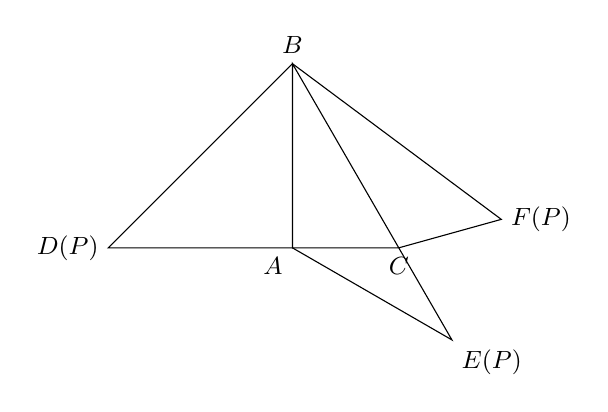
\begin{tikzpicture}[scale=1.35, font=\small]
  \coordinate (A) at (0,0);
  \coordinate (B) at (0,1.7320508);
  \coordinate (C) at (1,0);
  \coordinate (D) at (-1.7320508,0);
  \coordinate (E) at (1.5,-0.8660254);   % √3·(cos(-30°),sin(-30°))
  \coordinate (F) at (1.9641,0.2679);    % 由 FC=EC=1、FB=DB=√6 解出
  \draw (A) -- (B) -- (C) -- cycle;      % 中心三角形（折痕）
  \draw (B) -- (D) -- (A);               % △DAB
  \draw (A) -- (E) -- (C);               % △AEC
  \draw (C) -- (F) -- (B);               % △CFB
  \node[below left]  at (A) {$A$};
  \node[above]       at (B) {$B$};
  \node[below]       at (C) {$C$};
  \node[left]        at (D) {$D(P)$};
  \node[below right] at (E) {$E(P)$};
  \node[right]       at (F) {$F(P)$};
\end{tikzpicture}
\end{center}
\nopagebreak[4]
\Needspace{4\baselineskip}
\textbf{解析}

\textbf{第一步（本题的关键认知）：读懂展开图。}

图中标注了 $D(P)$、$E(P)$、$F(P)$，意思是\textbf{折叠还原成三棱锥后，$D$、$E$、$F$ 三点重合于顶点 $P$}。

\Needspace{5\baselineskip}
因此展开图上的线段与还原后的棱有如下对应：
\nopagebreak[4]
\[BD\ \longrightarrow\ PB,\qquad CE\ \longrightarrow\ PC,\qquad CF\ \longrightarrow\ PC\]

\Needspace{5\baselineskip}
而 $AD$、$AE$ 都对应 $PA$，所以
\nopagebreak[4]
\[AE=AD=\sqrt3\]

\Needspace{5\baselineskip}
\textbf{目标转化}：$\angle FCB$ 中的 $F$ 就是 $P$，故
\nopagebreak[4]
\[\cos\angle FCB=\cos\angle PCB\]

只需求出 $\triangle PCB$ 的三条边。

\par\medskip

\textbf{第二步，逐个计算三棱锥的棱长。}

\textbf{求 $PB$}（用展开图中的 $\triangle ABD$）：

\Needspace{5\baselineskip}
$AB=AD=\sqrt3$ 且 $AB\perp AD$，是等腰直角三角形：
\nopagebreak[4]
\[PB=BD=\sqrt{AB^{2}+AD^{2}}=\sqrt{3+3}=\sqrt6\]

\textbf{求 $PC$}（用展开图中的 $\triangle ACE$）：

\Needspace{5\baselineskip}
$AC=1$，$AE=\sqrt3$，$\angle CAE=30^\circ$，用余弦定理：
\nopagebreak[4]
\[CE^{2}=AC^{2}+AE^{2}-2\cdot AC\cdot AE\cos30^\circ=1+3-2\times1\times\sqrt3\times\frac{\sqrt3}2=4-3=1\]

\nopagebreak[4]
\[PC=CE=1\]

\textbf{求 $BC$}（用展开图中的 $\triangle ABC$）：

\Needspace{5\baselineskip}
$AB=\sqrt3$，$AC=1$，$AB\perp AC$：
\nopagebreak[4]
\[BC=\sqrt{3+1}=2\]

\par\medskip

\textbf{第三步，在 $\triangle PCB$ 中用余弦定理。}

\Needspace{5\baselineskip}
三边为 $PC=1$、$BC=2$、$PB=\sqrt6$：
\nopagebreak[4]
\[\cos\angle PCB=\frac{PC^{2}+BC^{2}-PB^{2}}{2\cdot PC\cdot BC}=\frac{1+4-6}{2\times1\times2}=\frac{-1}4=-\frac14\]

\begin{gktip}
\textbf{合理性检验}：$PC^{2}+BC^{2}=1+4=5<6=PB^{2}$，说明 $\angle PCB$ 是\textbf{钝角}，余弦为负  与结果一致。

\textbf{方法总结}：立体图形展开图问题的解法只有一句话——\textbf{先弄清哪些点在折叠后重合，把展开图上的长度"搬运"成立体图形中的棱长，再回到立体图形中用余弦定理}。展开图中的角度（如本题的 $\angle CAE=30^\circ$）只用于计算棱长，\textbf{不能直接当作立体图形中的角}。
\end{gktip}

\gkanswer{答案：$-\dfrac14$}

\par\medskip

\end{answer}
\gkpart{三、解答题}

\begin{answer}
\gksolhead{17}{12 分}

\textbf{题目}（12 分）：

设 $\left\{a_n\right\}$ 是公比不为 $1$ 的等比数列，$a_1$ 为 $a_2$，$a_3$ 的等差中项。

  (1) 求 $\left\{a_n\right\}$ 的公比；

  (2) 若 $a_1=1$，求数列 $\left\{na_n\right\}$ 的前 $n$ 项和。

\Needspace{4\baselineskip}
\textbf{解析}

\par\medskip

\textbf{(1) 解}

\Needspace{5\baselineskip}
"$a_1$ 为 $a_2$、$a_3$ 的等差中项"即
\nopagebreak[4]
\[2a_1=a_2+a_3\]

\Needspace{5\baselineskip}
设公比为 $q$，则 $a_2=a_1q$、$a_3=a_1q^{2}$：
\nopagebreak[4]
\[2a_1=a_1q+a_1q^{2}\]

\Needspace{5\baselineskip}
因等比数列首项 $a_1\ne0$，两边约去：
\nopagebreak[4]
\[q^{2}+q-2=0\ \Longrightarrow\ (q+2)(q-1)=0\]

\nopagebreak[4]
\[q=-2\qquad\text{\text{或}}\qquad q=1\]

\Needspace{5\baselineskip}
由题设"公比不为 $1$"，故
\nopagebreak[4]
\[q=-2\]

\par\medskip

\textbf{(2) 解}

\Needspace{5\baselineskip}
$a_1=1$，$q=-2$，故
\nopagebreak[4]
\[a_n=(-2)^{n-1},\qquad na_n=n(-2)^{n-1}\]

\Needspace{5\baselineskip}
记
\nopagebreak[4]
\[S_n=\sum_{k=1}^{n}k(-2)^{k-1}=1\times(-2)^{0}+2\times(-2)^{1}+3\times(-2)^{2}+\cdots+n(-2)^{n-1}\]

\Needspace{5\baselineskip}
\textbf{用错位相减法}（乘以公比 $-2$）：
\nopagebreak[4]
\[-2S_n=1\times(-2)^{1}+2\times(-2)^{2}+\cdots+(n-1)(-2)^{n-1}+n(-2)^{n}\]

\Needspace{5\baselineskip}
\textbf{两式相减}（上式减下式）：
\nopagebreak[4]
\[S_n-(-2)S_n=3S_n=\underbrace{(-2)^{0}+(-2)^{1}+(-2)^{2}+\cdots+(-2)^{n-1}}_{\text{\text{等比数列，}}n\ \text{\text{项}}}-n(-2)^{n}\]

\Needspace{5\baselineskip}
等比部分求和（首项 $1$、公比 $-2$）：
\nopagebreak[4]
\[\sum_{k=0}^{n-1}(-2)^{k}=\frac{1-(-2)^{n}}{1-(-2)}=\frac{1-(-2)^{n}}3\]

\Needspace{5\baselineskip}
于是
\nopagebreak[4]
\[3S_n=\frac{1-(-2)^{n}}3-n(-2)^{n}\]

\Needspace{5\baselineskip}
两边乘 $3$：
\nopagebreak[4]
\[9S_n=1-(-2)^{n}-3n(-2)^{n}=1-(3n+1)(-2)^{n}\]

\nopagebreak[4]
\[\boxed{S_n=\frac{1-(3n+1)(-2)^{n}}9}\]

\textbf{校验}（务必做）：
\begin{itemize}
\item $n=1$：$\dfrac{1-4\times(-2)}9=\dfrac{1+8}9=1$，而 $S_1=1\times a_1=1$ 
\item $n=2$：$\dfrac{1-7\times4}9=\dfrac{-27}9=-3$，而 $S_2=1+2\times(-2)=-3$ 
\end{itemize}

\begin{gktip}
\textbf{方法总结}：形如 $\{n\cdot q^{n}\}$（等差 × 等比）的求和一律用\textbf{错位相减}。步骤固定：① 写出 $S_n$；② 两边乘公比 $q$；③ 错位相减，中间变成等比数列求和；④ 解出 $S_n$；⑤ \textbf{代 $n=1,2$ 校验}。公比为负数时符号容易出错，校验尤其必要。
\end{gktip}

\gkanswer{答案（1）：$q=-2$}

\gkanswer{答案（2）：$S_n=\dfrac{1-(3n+1)(-2)^{n}}9$}

\par\medskip

\end{answer}
\begin{answer}
\gksolhead{18}{12 分}

\textbf{题目}（12 分）：

如图，$D$ 为圆锥的顶点，$O$ 是圆锥底面的圆心，$AE$ 为底面直径，$AE=AD$。$\triangle ABC$ 是底面的内接正三角形，$P$ 为 $DO$ 上一点，$PO=\dfrac{\sqrt6}6DO$。
\nopagebreak[4]
\begin{center}% 2020 全国Ⅰ卷 理18：圆锥（顶点 D，底面圆心 O，AE 为直径，△ABC 内接正三角形，P 在 DO 上）
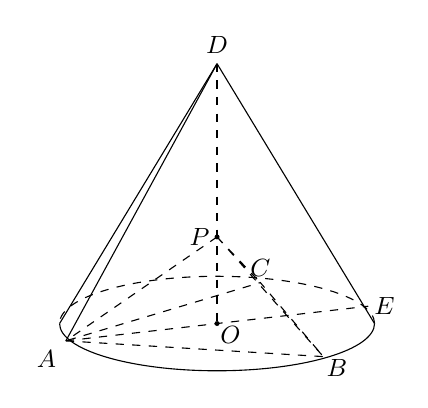
\begin{tikzpicture}[scale=1.0, font=\small]
  \coordinate (D) at (0,3.3);
  \coordinate (O) at (0,0);
  \coordinate (A) at (-1.92,-0.22);
  \coordinate (E) at (1.92,0.22);
  \coordinate (B) at (1.35,-0.42);
  \coordinate (C) at (0.55,0.52);
  \coordinate (P) at (0,1.1);
  % 底面椭圆：前半实、后半虚
  \draw (-2,0) arc (180:360:2 and 0.6);
  \draw[dashed] (2,0) arc (0:180:2 and 0.6);
  % 锥面轮廓
  \draw (D) -- (-2,0);
  \draw (D) -- (2,0);
  % 中轴与内部连线
  \draw[dashed] (D) -- (O);
  \draw[dashed] (A) -- (E);
  \draw[dashed] (A) -- (B) -- (C) -- cycle;
  \draw[dashed] (P) -- (A)  (P) -- (B)  (P) -- (C);
  \draw (D) -- (A);
  \fill (O) circle (0.9pt);  \fill (P) circle (0.9pt);
  \node[above] at (D) {$D$};
  \node[below left] at (A) {$A$};
  \node[below right, inner sep=1pt] at (B) {$B$};
  \node[right, inner sep=2pt] at (E) {$E$};
  \node[above, inner sep=2pt] at (C) {$C$};
  \node[below right, inner sep=1pt] at (O) {$O$};
  \node[left, inner sep=2.5pt] at (P) {$P$};
\end{tikzpicture}
\end{center}
\nopagebreak[4]
  (1) 证明：$PA\perp$ 平面 $PBC$；

  (2) 求二面角 $B\text{-}PC\text{-}E$ 的余弦值。

\Needspace{4\baselineskip}
\textbf{解析}

  (1) 证明：$PA\perp$ 平面 $PBC$；(2) 求二面角 $B\text{-}PC\text{-}E$ 的余弦值。

\par\medskip

\textbf{建系（两问共用）}

设底面半径为 $1$（比例问题，可自由设定）。

由 $AE=AD$ 且 $AE$ 是直径：$AD=2$，即母线长为 $2$。

\Needspace{5\baselineskip}
圆锥的高：
\nopagebreak[4]
\[DO=\sqrt{AD^{2}-AO^{2}}=\sqrt{4-1}=\sqrt3\]

\nopagebreak[4]
\[PO=\frac{\sqrt6}6\times\sqrt3=\frac{\sqrt{18}}6=\frac{3\sqrt2}6=\frac{\sqrt2}2\]

\Needspace{5\baselineskip}
以 $O$ 为原点、$AE$ 所在直线为 $x$ 轴、$OD$ 为 $z$ 轴建系。$\triangle ABC$ 为底面内接正三角形，$A$ 在 $x$ 轴负方向：
\nopagebreak[4]
\[O(0,0,0),\quad A(-1,0,0),\quad E(1,0,0),\quad P\left(0,0,\frac{\sqrt2}2\right)\]

\Needspace{5\baselineskip}
$B$、$C$ 与 $A$ 相差 $\pm120^\circ$：
\nopagebreak[4]
\[B\left(\frac12,\ -\frac{\sqrt3}2,\ 0\right),\qquad C\left(\frac12,\ \frac{\sqrt3}2,\ 0\right)\]

\par\medskip

\Needspace{5\baselineskip}
\textbf{(1) 证明}

\nopagebreak[4]
\[\overrightarrow{PA}=A-P=\left(-1,\ 0,\ -\frac{\sqrt2}2\right)\]
\nopagebreak[4]
\[\overrightarrow{PB}=B-P=\left(\frac12,\ -\frac{\sqrt3}2,\ -\frac{\sqrt2}2\right),\qquad \overrightarrow{PC}=C-P=\left(\frac12,\ \frac{\sqrt3}2,\ -\frac{\sqrt2}2\right)\]

\Needspace{5\baselineskip}
\textbf{逐个验证数量积}：
\nopagebreak[4]
\[\overrightarrow{PA}\cdot\overrightarrow{PB}=(-1)\times\frac12+0\times\left(-\frac{\sqrt3}2\right)+\left(-\frac{\sqrt2}2\right)\times\left(-\frac{\sqrt2}2\right)=-\frac12+0+\frac12=0\]

\nopagebreak[4]
\[\overrightarrow{PA}\cdot\overrightarrow{PC}=(-1)\times\frac12+0\times\frac{\sqrt3}2+\left(-\frac{\sqrt2}2\right)\times\left(-\frac{\sqrt2}2\right)=-\frac12+\frac12=0\]

\Needspace{5\baselineskip}
故
\nopagebreak[4]
\[PA\perp PB,\qquad PA\perp PC\]

\Needspace{5\baselineskip}
又 $PB$ 与 $PC$ 是平面 $PBC$ 内的\textbf{两条相交直线}（交于 $P$），由线面垂直的判定定理：
\nopagebreak[4]
\[PA\perp\text{\text{平面} }PBC\qquad\blacksquare\]

\begin{gktip}
\textbf{注意 $PO=\dfrac{\sqrt6}6DO$ 这个奇怪的比例正是为了让上面两个数量积恰好为零}——命题人反推设计的结果。
\end{gktip}

\par\medskip

\textbf{(2) 解}

\Needspace{5\baselineskip}
\textbf{省力技巧}：由 (1) 的结论，$\overrightarrow{PA}$ \textbf{本身就是平面 $PBC$ 的法向量}，不必再算叉乘！
\nopagebreak[4]
\[\boldsymbol n_1=\overrightarrow{PA}=\left(-1,\ 0,\ -\frac{\sqrt2}2\right),\qquad \left|\boldsymbol n_1\right|=\sqrt{1+\frac12}=\frac{\sqrt6}2\]

\Needspace{5\baselineskip}
\textbf{求平面 $EPC$ 的法向量}：
\nopagebreak[4]
\[\overrightarrow{PE}=E-P=\left(1,\ 0,\ -\frac{\sqrt2}2\right),\qquad \overrightarrow{PC}=\left(\frac12,\ \frac{\sqrt3}2,\ -\frac{\sqrt2}2\right)\]

\nopagebreak[4]
\[\boldsymbol n_2=\overrightarrow{PE}\times\overrightarrow{PC}=\begin{vmatrix}\boldsymbol i&\boldsymbol j&\boldsymbol k\\ 1&0&-\frac{\sqrt2}2\\ \frac12&\frac{\sqrt3}2&-\frac{\sqrt2}2\end{vmatrix}\]

逐分量计算：
\begin{itemize}
\item $\boldsymbol i$：$0\times\left(-\dfrac{\sqrt2}2\right)-\left(-\dfrac{\sqrt2}2\right)\times\dfrac{\sqrt3}2=\dfrac{\sqrt6}4$
\item $\boldsymbol j$：$-\left[1\times\left(-\dfrac{\sqrt2}2\right)-\left(-\dfrac{\sqrt2}2\right)\times\dfrac12\right]=-\left(-\dfrac{\sqrt2}2+\dfrac{\sqrt2}4\right)=\dfrac{\sqrt2}4$
\item $\boldsymbol k$：$1\times\dfrac{\sqrt3}2-0\times\dfrac12=\dfrac{\sqrt3}2$
\end{itemize}

\nopagebreak[4]
\[\boldsymbol n_2=\left(\frac{\sqrt6}4,\ \frac{\sqrt2}4,\ \frac{\sqrt3}2\right)\]

\nopagebreak[4]
\[\left|\boldsymbol n_2\right|=\sqrt{\frac6{16}+\frac2{16}+\frac34}=\sqrt{\frac{6+2+12}{16}}=\sqrt{\frac{20}{16}}=\frac{\sqrt5}2\]

\Needspace{5\baselineskip}
\textbf{取垂直于棱 $PC$ 的截面}：平面 $PBC$ 中由 $P$ 指向 $B$ 的方向已经垂直于 $PC$，记
\nopagebreak[4]
\[\boldsymbol u=\overrightarrow{PB}=\left(\frac12,-\frac{\sqrt3}2,-\frac{\sqrt2}2\right).\]

\Needspace{5\baselineskip}
将 $\overrightarrow{PE}$ 投影到 $PC^\perp$，得到平面 $PCE$ 中指向 $E$ 的截面方向
\nopagebreak[4]
\[\boldsymbol v=\overrightarrow{PE}-\frac{\overrightarrow{PE}\cdot\overrightarrow{PC}}{|\overrightarrow{PC}|^2}\overrightarrow{PC}=\left(\frac23,-\frac{\sqrt3}3,-\frac{\sqrt2}6\right).\]

\Needspace{5\baselineskip}
其中 $\boldsymbol u\cdot\boldsymbol v=1$，$|\boldsymbol u|=\frac{\sqrt6}2$，$|\boldsymbol v|=\sqrt{\frac56}$。这两条向量分别指向题设两半平面在截面中的方向，故二面角为锐角，
\nopagebreak[4]
\[\cos\theta=\frac{\boldsymbol u\cdot\boldsymbol v}{|\boldsymbol u||\boldsymbol v|}=\frac{2}{\sqrt5}=\frac{2\sqrt5}5.\]

\begin{gktip}
\textbf{方法总结}：本题体现了"\textbf{前一问的结论是后一问的工具}"这一常见设计——第 (1) 问证明的 $PA\perp$ 平面 $PBC$，直接提供了第 (2) 问所需的一个法向量，省去一次叉乘运算。做立体几何解答题时，先做完 (1) 再看 (2)，往往能发现这种"馈赠"。
\end{gktip}

\gkanswer{答案（1）：见解析版}

\gkanswer{答案（2）：$\dfrac{2\sqrt5}5$}

\par\medskip

\end{answer}
\begin{answer}
\gksolhead{19}{12 分}

\textbf{题目}（12 分）：

甲、乙、丙三位同学进行羽毛球比赛，约定赛制如下：累计负两场者被淘汰；比赛前抽签决定首先比赛的两人，另一人轮空；每场比赛的胜者与轮空者进行下一场比赛，负者下一场轮空，直至有一人被淘汰；当一人被淘汰后，剩余的两人继续比赛，直至其中一人被淘汰，另一人最终获胜，比赛结束。经抽签，甲、乙首先比赛，丙轮空。设每场比赛双方获胜的概率都为 $\dfrac12$。

  (1) 求甲连胜四场的概率；

  (2) 求需要进行第五场比赛的概率；

  (3) 求丙最终获胜的概率。

\Needspace{4\baselineskip}
\textbf{解析}

\par\medskip

\textbf{赛制梳理（做题前必须理清）}

\begin{itemize}
\item 场 1：甲 vs 乙（丙轮空）
\item 场 2：场 1 的胜者 vs 丙（场 1 的负者轮空）
\item 场 3：场 2 的胜者 vs 场 1 的负者
\item 以此类推，直到有人累计负两场被淘汰；两人被淘汰后剩下的人获胜
\end{itemize}

\par\medskip

\textbf{(1) 解}

\Needspace{5\baselineskip}
甲连胜四场，即甲在场 1、2、3、4 中全部获胜。各场独立且胜率均为 $\dfrac12$：
\nopagebreak[4]
\[P=\left(\frac12\right)^{4}=\frac1{16}\]

\textbf{验证这确实意味着比赛结束}：甲胜场 1（乙负 1）、胜场 2（丙负 1）、胜场 3（乙负 2，淘汰）、胜场 4（丙负 2，淘汰）——两人都被淘汰，甲最终获胜 

\par\medskip

\textbf{(2) 解}

\textbf{思路：先求"四场就结束"的概率，再取补集。}

四场比赛共产生 $4$ 个负场。比赛在四场内结束，意味着这 $4$ 个负场恰好由\textbf{两个人各承担 $2$ 场}（他们都被淘汰）。

\textbf{穷举所有可能：}

1. \textbf{甲连胜四场}：乙负 $2$、丙负 $2$  概率 $\dfrac1{16}$
2. \textbf{乙连胜四场}：对称  概率 $\dfrac1{16}$
3. \textbf{甲胜场 1，丙连胜场 2、3、4}：
\begin{itemize}
\item 场 1 甲胜（乙负 1）
\item 场 2 丙胜（甲负 1）
\item 场 3 丙 vs 乙，丙胜（乙负 2，淘汰）
\item 场 4 丙 vs 甲，丙胜（甲负 2，淘汰） 概率 $\left(\dfrac12\right)^{4}=\dfrac1{16}$
\end{itemize}
4. \textbf{乙胜场 1，丙连胜场 2、3、4}：对称  概率 $\dfrac1{16}$

（丙无法"连胜四场"，因为他场 1 轮空，最多参加场 2、3、4 三场。）

\Needspace{5\baselineskip}
\textbf{四场结束的概率}：
\nopagebreak[4]
\[P_4=4\times\frac1{16}=\frac14\]

\Needspace{5\baselineskip}
\textbf{需要第五场的概率}：
\nopagebreak[4]
\[P=1-\frac14=\frac34\]

\par\medskip

\textbf{(3) 解}

\Needspace{5\baselineskip}
由甲、乙\textbf{地位对称}（都在场 1 出战），丙的获胜概率与"场 1 谁胜"无关。不妨设\textbf{场 1 甲胜}，此时状态为：

\nopagebreak[4]
\[\text{\text{负场数}}(\text{\text{甲}},\text{\text{乙}},\text{\text{丙}})=(0,1,0),\qquad \text{\text{场} 2\text{：甲} vs \text{丙}}\]

\textbf{分支一：场 2 甲胜}（概率 $\dfrac12$），状态 $(0,1,1)$，场 3 甲 vs 乙

\begin{itemize}
\item \textbf{甲胜场 3}（$\dfrac12$）：乙负 $2$ 淘汰，剩甲（$0$ 负）、丙（$1$ 负）。场 4 甲 vs 丙：
\item 甲胜（$\dfrac12$）：丙负 $2$，甲获胜 → 丙失败
\item 丙胜（$\dfrac12$）：甲负 $1$，场 5 甲 vs 丙 → 丙以 $\dfrac12$ 获胜
\end{itemize}

  丙获胜概率 $=\dfrac12\times\dfrac12=\dfrac14$

\begin{itemize}
\item \textbf{乙胜场 3}（$\dfrac12$）：甲负 $1$，状态 $(1,1,1)$，场 4 乙 vs 丙：
\item 乙胜（$\dfrac12$）：丙负 $2$ 淘汰 → 丙失败
\item 丙胜（$\dfrac12$）：乙负 $2$ 淘汰，场 5 丙 vs 甲 → 丙以 $\dfrac12$ 获胜
\end{itemize}

  丙获胜概率 $=\dfrac12\times\dfrac12=\dfrac14$

\Needspace{5\baselineskip}
\textbf{分支一中丙获胜的概率}：
\nopagebreak[4]
\[\frac12\times\frac14+\frac12\times\frac14=\frac14\]

\par\medskip

\textbf{分支二：场 2 丙胜}（概率 $\dfrac12$），状态 $(1,1,0)$，场 3 丙 vs 乙

\begin{itemize}
\item \textbf{丙胜场 3}（$\dfrac12$）：乙负 $2$ 淘汰，剩丙（$0$ 负）、甲（$1$ 负）。场 4 丙 vs 甲：
\item 丙胜（$\dfrac12$）：甲负 $2$，\textbf{丙获胜} 
\item 甲胜（$\dfrac12$）：丙负 $1$，场 5 → 丙以 $\dfrac12$ 获胜
\end{itemize}

  丙获胜概率 $=\dfrac12+\dfrac12\times\dfrac12=\dfrac34$

\begin{itemize}
\item \textbf{乙胜场 3}（$\dfrac12$）：丙负 $1$，状态 $(1,1,1)$，场 4 乙 vs 甲：
\item 无论谁胜，都有一人负 $2$ 被淘汰，剩下的人与丙打场 5，丙以 $\dfrac12$ 获胜
\end{itemize}

  丙获胜概率 $=\dfrac12$

\Needspace{5\baselineskip}
\textbf{分支二中丙获胜的概率}：
\nopagebreak[4]
\[\frac12\times\frac34+\frac12\times\frac12=\frac38+\frac14=\frac58\]

\par\medskip

\Needspace{5\baselineskip}
\textbf{综合}：
\nopagebreak[4]
\[P(\text{\text{丙获胜}})=\frac12\times\frac14+\frac12\times\frac58=\frac18+\frac5{16}=\frac2{16}+\frac5{16}=\frac7{16}\]

\begin{gktip}
\textbf{合理性检验}：由对称性 $P(\text{\text{甲}})=P(\text{\text{乙}})=\dfrac12\left(1-\dfrac7{16}\right)=\dfrac9{32}$。
注意 $\dfrac7{16}=\dfrac{14}{32}>\dfrac9{32}$，即\textbf{丙的获胜概率最大}！

\textbf{这个反直觉的结果值得向学生强调}：丙第一场轮空看似"少了一次表现机会"，实则\textbf{少了一次输球的机会}——在"负两场淘汰"的赛制下，避免早期风险比多打一场更有价值。这是概率论中"策略优势"的一个漂亮例子。
\end{gktip}

\gkanswer{答案（1）：$\dfrac1{16}$}

\gkanswer{答案（2）：$\dfrac34$}

\gkanswer{答案（3）：$\dfrac7{16}$}

\par\medskip

\end{answer}
\begin{answer}
\gksolhead{20}{12 分}

\textbf{题目}（12 分）：

已知 $A$，$B$ 分别为椭圆 $E:\dfrac{x^{2}}{a^{2}}+y^{2}=1\ (a>1)$ 的左、右顶点，$G$ 为 $E$ 的上顶点，$\overrightarrow{AG}\cdot\overrightarrow{GB}=8$，$P$ 为直线 $x=6$ 上的动点，$PA$ 与 $E$ 的另一交点为 $C$，$PB$ 与 $E$ 的另一交点为 $D$。

  (1) 求 $E$ 的方程；

  (2) 证明：直线 $CD$ 过定点。

\Needspace{4\baselineskip}
\textbf{解析}

\par\medskip

\textbf{(1) 解}

\Needspace{5\baselineskip}
由椭圆方程，$b=1$，三个顶点为
\nopagebreak[4]
\[A(-a,\ 0),\qquad B(a,\ 0),\qquad G(0,\ 1)\]

\nopagebreak[4]
\[\overrightarrow{AG}=G-A=(a,\ 1),\qquad \overrightarrow{GB}=B-G=(a,\ -1)\]

\nopagebreak[4]
\[\overrightarrow{AG}\cdot\overrightarrow{GB}=a^{2}-1=8\ \Longrightarrow\ a^{2}=9\]

（$a=3>1$  符合题设。）

\Needspace{5\baselineskip}
\textbf{所以 $E$ 的方程为}
\nopagebreak[4]
\[\frac{x^{2}}9+y^{2}=1\]

\par\medskip

\textbf{(2) 证明}

此时 $A(-3,0)$、$B(3,0)$。设 $P(6,\ t)$（$t\ne0$，否则 $C$、$D$ 退化）。

\textbf{第一步，求 $C$ 的坐标（用"已知一根"的因式分解技巧）。}

\Needspace{5\baselineskip}
直线 $PA$ 过 $A(-3,0)$ 与 $P(6,t)$，斜率 $\dfrac t9$：
\nopagebreak[4]
\[y=\frac t9(x+3)\]

\Needspace{5\baselineskip}
代入椭圆（写成 $x^{2}+9y^{2}=9$）：
\nopagebreak[4]
\[x^{2}+9\times\frac{t^{2}}{81}(x+3)^{2}=9\ \Longrightarrow\ 9x^{2}+t^{2}(x+3)^{2}=81\]

\Needspace{5\baselineskip}
\textbf{关键：把常数项移过来配成含 $(x+3)$ 的因式}：
\nopagebreak[4]
\[9\left(x^{2}-9\right)+t^{2}(x+3)^{2}=0\ \Longrightarrow\ 9(x-3)(x+3)+t^{2}(x+3)^{2}=0\]

\nopagebreak[4]
\[(x+3)\left[9(x-3)+t^{2}(x+3)\right]=0\]

\Needspace{5\baselineskip}
一根为 $x=-3$（即点 $A$），另一根：
\nopagebreak[4]
\[\left(9+t^{2}\right)x=27-3t^{2}\ \Longrightarrow\ x_C=\frac{27-3t^{2}}{9+t^{2}}\]

\nopagebreak[4]
\[y_C=\frac t9\left(x_C+3\right)=\frac t9\times\frac{27-3t^{2}+27+3t^{2}}{9+t^{2}}=\frac t9\times\frac{54}{9+t^{2}}=\frac{6t}{9+t^{2}}\]

\textbf{第二步，同法求 $D$。}

\Needspace{5\baselineskip}
直线 $PB$ 过 $B(3,0)$ 与 $P(6,t)$，斜率 $\dfrac t3$：
\nopagebreak[4]
\[y=\frac t3(x-3)\]

\Needspace{5\baselineskip}
代入 $x^{2}+9y^{2}=9$：
\nopagebreak[4]
\[x^{2}+t^{2}(x-3)^{2}=9\ \Longrightarrow\ (x-3)(x+3)+t^{2}(x-3)^{2}=0\]

\nopagebreak[4]
\[(x-3)\left[(x+3)+t^{2}(x-3)\right]=0\]

\Needspace{5\baselineskip}
另一根：
\nopagebreak[4]
\[\left(1+t^{2}\right)x=3t^{2}-3\ \Longrightarrow\ x_D=\frac{3\left(t^{2}-1\right)}{t^{2}+1}\]

\nopagebreak[4]
\[y_D=\frac t3\left(x_D-3\right)=\frac t3\times\frac{3t^{2}-3-3t^{2}-3}{t^{2}+1}=\frac t3\times\frac{-6}{t^{2}+1}=\frac{-2t}{t^{2}+1}\]

\textbf{第三步，求直线 $CD$ 的斜率。}

\Needspace{5\baselineskip}
\textbf{分子}：
\nopagebreak[4]
\[y_C-y_D=\frac{6t}{9+t^{2}}+\frac{2t}{1+t^{2}}=2t\cdot\frac{3\left(1+t^{2}\right)+\left(9+t^{2}\right)}{\left(9+t^{2}\right)\left(1+t^{2}\right)}=\frac{2t\left(4t^{2}+12\right)}{\left(9+t^{2}\right)\left(1+t^{2}\right)}=\frac{8t\left(t^{2}+3\right)}{\left(9+t^{2}\right)\left(1+t^{2}\right)}\]

\Needspace{5\baselineskip}
\textbf{分母}：
\nopagebreak[4]
\[x_C-x_D=\frac{\left(27-3t^{2}\right)\left(1+t^{2}\right)-\left(3t^{2}-3\right)\left(9+t^{2}\right)}{\left(9+t^{2}\right)\left(1+t^{2}\right)}\]

\Needspace{5\baselineskip}
分子展开：
\nopagebreak[4]
\[\left(27+24t^{2}-3t^{4}\right)-\left(24t^{2}+3t^{4}-27\right)=54-6t^{4}=6\left(9-t^{4}\right)=6\left(3-t^{2}\right)\left(3+t^{2}\right)\]

\Needspace{5\baselineskip}
\textbf{相除（公分母约去）}：
\nopagebreak[4]
\[k_{CD}=\frac{8t\left(t^{2}+3\right)}{6\left(3-t^{2}\right)\left(3+t^{2}\right)}=\frac{8t}{6\left(3-t^{2}\right)}=\frac{4t}{3\left(3-t^{2}\right)}\]

\textbf{第四步，求 $CD$ 与 $x$ 轴的交点（猜测定点在 $x$ 轴上）。}

\Needspace{5\baselineskip}
由点斜式，令 $y=0$：
\nopagebreak[4]
\[x=x_D-\frac{y_D}{k_{CD}}=\frac{3\left(t^{2}-1\right)}{t^{2}+1}-\frac{\dfrac{-2t}{t^{2}+1}}{\dfrac{4t}{3\left(3-t^{2}\right)}}\]

\nopagebreak[4]
\[=\frac{3\left(t^{2}-1\right)}{t^{2}+1}+\frac{2t}{t^{2}+1}\times\frac{3\left(3-t^{2}\right)}{4t}=\frac{3\left(t^{2}-1\right)}{t^{2}+1}+\frac{3\left(3-t^{2}\right)}{2\left(t^{2}+1\right)}\]

\Needspace{5\baselineskip}
通分：
\nopagebreak[4]
\[=\frac{6\left(t^{2}-1\right)+3\left(3-t^{2}\right)}{2\left(t^{2}+1\right)}=\frac{6t^{2}-6+9-3t^{2}}{2\left(t^{2}+1\right)}=\frac{3t^{2}+3}{2\left(t^{2}+1\right)}=\frac{3\left(t^{2}+1\right)}{2\left(t^{2}+1\right)}=\frac32\]

\textbf{结果与 $t$ 完全无关！}

\textbf{所以直线 $CD$ 恒过定点 $\left(\dfrac32,\ 0\right)$。$\blacksquare$}

\begin{gktip}
\textbf{方法总结}：本题有两个关键技巧——
① \textbf{"已知一根"的因式分解}：直线过椭圆上的已知点（顶点 $A$ 或 $B$）时，联立方程必有一根是该点的横坐标，因此可以直接\textbf{配出因式} $(x+3)$ 或 $(x-3)$，避免解二次方程。这比用韦达定理更直接。
② \textbf{定点问题的验证路径}：算出直线与坐标轴的交点，若结果\textbf{不含参数}，即证明了过定点。若不确定定点在哪条轴上，可先取两个特殊的 $t$ 值求出两条具体的直线，交点即为猜测的定点，再一般化证明。
\end{gktip}

\gkanswer{答案（1）：$\dfrac{x^{2}}9+y^{2}=1$}

\gkanswer{答案（2）：直线 $CD$ 过定点 $\left(\dfrac32,\ 0\right)$}

\par\medskip

\end{answer}
\begin{answer}
\gksolhead{21}{12 分}

\textbf{题目}（12 分）：

已知函数 $f(x)=\mathrm e^{x}+ax^{2}-x$。

  (1) 当 $a=1$ 时，讨论 $f(x)$ 的单调性；

  (2) 当 $x\ge0$ 时，$f(x)\ge\dfrac12x^{3}+1$，求 $a$ 的取值范围。

\Needspace{4\baselineskip}
\textbf{解析}

\par\medskip

\textbf{(1) 解}

\Needspace{5\baselineskip}
$a=1$ 时 $f(x)=\mathrm e^{x}+x^{2}-x$。
\nopagebreak[4]
\[f'(x)=\mathrm e^{x}+2x-1\]

\Needspace{5\baselineskip}
\textbf{关键：$f'$ 本身还含超越项，需要再求一次导。}
\nopagebreak[4]
\[f''(x)=\mathrm e^{x}+2>0\qquad\text{\text{恒成立}}\]

故 $f'(x)$ 在 $\mathbf R$ 上\textbf{严格递增}。

\Needspace{5\baselineskip}
又
\nopagebreak[4]
\[f'(0)=\mathrm e^{0}+0-1=0\]

因此 $f'$ 有唯一零点 $x=0$：
\begin{itemize}
\item $x<0$ 时 $f'(x)<f'(0)=0$，$f$ 单调递减
\item $x>0$ 时 $f'(x)>0$，$f$ 单调递增
\end{itemize}

\textbf{结论}：$f(x)$ 在 $(-\infty,\ 0)$ 上单调递减，在 $(0,\ +\infty)$ 上单调递增。

\par\medskip

\textbf{(2) 解}

\textbf{第一步，观察 $x=0$。}

\Needspace{5\baselineskip}
原不等式为
\nopagebreak[4]
\[\mathrm e^{x}+ax^{2}-x\ge\frac12x^{3}+1\]

$x=0$ 时两边都等于 $1$，\textbf{取等号}，对 $a$ 无约束。

\textbf{第二步，对 $x>0$ 分离参数。}

\Needspace{5\baselineskip}
移项：
\nopagebreak[4]
\[ax^{2}\ge\frac12x^{3}+1+x-\mathrm e^{x}\]

\Needspace{5\baselineskip}
因 $x>0$ 故 $x^{2}>0$，两边同除以 $x^{2}$（不等号方向不变）：
\nopagebreak[4]
\[a\ge\varphi(x)\ \overset{\text{\text{记}}}{=}\ \frac{\dfrac12x^{3}+x+1-\mathrm e^{x}}{x^{2}}\]

\textbf{问题转化为}：求 $\varphi(x)$ 在 $(0,+\infty)$ 上的\textbf{最大值}。

\textbf{第三步，求导。}

\Needspace{5\baselineskip}
把 $\varphi$ 拆开便于求导：
\nopagebreak[4]
\[\varphi(x)=\frac x2+\frac{x+1-\mathrm e^{x}}{x^{2}}\]

\nopagebreak[4]
\[\varphi'(x)=\frac12+\frac{\left(1-\mathrm e^{x}\right)x^{2}-\left(x+1-\mathrm e^{x}\right)\cdot2x}{x^{4}}=\frac12+\frac{\left(1-\mathrm e^{x}\right)x-2\left(x+1-\mathrm e^{x}\right)}{x^{3}}\]

\Needspace{5\baselineskip}
分子整理：
\nopagebreak[4]
\[x-x\mathrm e^{x}-2x-2+2\mathrm e^{x}=-x-2+\mathrm e^{x}(2-x)\]

\Needspace{5\baselineskip}
于是
\nopagebreak[4]
\[\varphi'(x)=\frac{\dfrac{x^{3}}2+\mathrm e^{x}(2-x)-x-2}{x^{3}}\ \overset{\text{\text{记}}}{=}\ \frac{\psi(x)}{x^{3}}\]

因 $x>0$ 时 $x^{3}>0$，$\varphi'$ 与 $\psi$ \textbf{同号}。

\textbf{第四步，分析 $\psi(x)=\dfrac{x^{3}}2+\mathrm e^{x}(2-x)-x-2$。}

\Needspace{5\baselineskip}
\textbf{先找特殊零点}：
\nopagebreak[4]
\[\psi(0)=0+2-0-2=0\]
\nopagebreak[4]
\[\psi(2)=4+\mathrm e^{2}\times0-2-2=0\]

\textbf{两个零点 $x=0$ 与 $x=2$。}

\Needspace{5\baselineskip}
\textbf{再看 $\psi$ 的导数}：
\nopagebreak[4]
\[\psi'(x)=\frac{3x^{2}}2+\mathrm e^{x}(2-x)-\mathrm e^{x}-1=\frac{3x^{2}}2+\mathrm e^{x}(1-x)-1\]

\nopagebreak[4]
\[\psi''(x)=3x+\mathrm e^{x}(1-x)-\mathrm e^{x}=3x-x\mathrm e^{x}=x\left(3-\mathrm e^{x}\right)\]

$\psi''$ 的零点：$x=0$ 或 $\mathrm e^{x}=3$ 即 $x=\ln3\approx1.099$。

\begin{itemize}
\item $0<x<\ln3$：$\psi''>0$，$\psi'$ 递增
\item $x>\ln3$：$\psi''<0$，$\psi'$ 递减
\end{itemize}

又 $\psi'(0)=0+1-1=0$，$\psi'(2)=6+\mathrm e^{2}\times(-1)-1=5-\mathrm e^{2}\approx-2.39<0$。

故 $\psi'$ 在 $(0,\ln3)$ 上由 $0$ 增到正值，在 $(\ln3,+\infty)$ 上递减并在某点 $x_0\in(\ln3,2)$ 变号。

\Needspace{5\baselineskip}
\textbf{综合得 $\psi$ 的符号}：$\psi$ 在 $(0,x_0)$ 递增（从 $\psi(0)=0$ 开始），在 $(x_0,+\infty)$ 递减，而 $\psi(2)=0$，因此
\nopagebreak[4]
\[\psi(x)>0\ \text{\text{在}}\ (0,2);\qquad \psi(x)<0\ \text{\text{在}}\ (2,+\infty)\]

\textbf{第五步，得出 $\varphi$ 的最大值。}

\Needspace{5\baselineskip}
$\varphi'>0$ 在 $(0,2)$、$\varphi'<0$ 在 $(2,+\infty)$，故 $\varphi$ 在 $x=2$ 处取得\textbf{最大值}：
\nopagebreak[4]
\[\varphi(2)=\frac{\dfrac12\times8+2+1-\mathrm e^{2}}{4}=\frac{4+3-\mathrm e^{2}}4=\frac{7-\mathrm e^{2}}4\]

\Needspace{5\baselineskip}
\textbf{第六步，结论。}
\nopagebreak[4]
\[a\ge\frac{7-\mathrm e^{2}}4\]

（数值上 $\mathrm e^{2}\approx7.389$，故 $\dfrac{7-\mathrm e^{2}}4\approx-0.097$。）

\begin{gktip}
\textbf{方法总结}："恒成立求参数"的标准路线是\textbf{分离参数 → 求另一侧函数的最值}。本题的难点在于分离后的 $\varphi(x)$ 求导很复杂，需要\textbf{二次甚至三次求导}才能确定符号。技巧是：把 $\varphi'$ 写成 $\dfrac{\psi(x)}{x^{3}}$ 的形式后，只研究分子 $\psi$；发现 $\psi$ 有"漂亮"的零点 $x=0$ 与 $x=2$，正是命题人埋的路标——\textbf{看到 $\psi(2)=0$ 这样的巧合，基本可以确定 $x=2$ 就是最值点}。
\end{gktip}

\gkanswer{答案（1）：$f'(x)=\mathrm e^{x}+2x-1$，$f''(x)=\mathrm e^{x}+2>0$ 故 $f'$ 严格递增，又 $f'(0)=0$，所以 $f$ 在 $(-\infty,0)$ 递减、在 $(0,+\infty)$ 递增。}

\gkanswer{答案（2）：$a\ge\dfrac{7-\mathrm e^{2}}4$}

\par\medskip

\end{answer}
\gkpart{四、选考题（现行考纲已取消，仅存档）}

\begin{gktip}
以下两题的内容（极坐标与参数方程、不等式选讲）已从新课标中删除，\textbf{不建议练习}，此处仅作历史资料保留，解析从简。
\end{gktip}

\begin{answer}
\gksolhead{22}{坐标系与参数方程}

\textbf{题目}（10 分）〔选修 4-4：坐标系与参数方程〕：

（\textbf{已取消}）

在直角坐标系 $xOy$ 中，曲线 $C_1$ 的参数方程为 $\begin{cases}x=\cos^{k}t\\ y=\sin^{k}t\end{cases}$（$t$ 为参数）。以坐标原点为极点，$x$ 轴正半轴为极轴建立极坐标系，曲线 $C_2$ 的极坐标方程为 $4\rho\cos\theta-16\rho\sin\theta+3=0$。

  (1) 当 $k=1$ 时，$C_1$ 是什么曲线？

  (2) 当 $k=4$ 时，求 $C_1$ 与 $C_2$ 的公共点的直角坐标。

\Needspace{4\baselineskip}
\textbf{解析}

\Needspace{5\baselineskip}
\textbf{(1)}　$k=1$ 时 $\begin{cases}x=\cos t\\ y=\sin t\end{cases}$，消参得
\nopagebreak[4]
\[x^{2}+y^{2}=1\]

即\textbf{以原点为圆心、半径为 $1$ 的圆}。

\Needspace{5\baselineskip}
\textbf{(2)}　$k=4$ 时 $x=\cos^{4}t$、$y=\sin^{4}t$，故 $\sqrt x=\cos^{2}t$、$\sqrt y=\sin^{2}t$，由 $\cos^2t+\sin^2t=1$：
\nopagebreak[4]
\[C_1:\ \sqrt x+\sqrt y=1\qquad(x,y\ge0)\]

\Needspace{5\baselineskip}
$C_2$ 的极坐标方程 $4\rho\cos\theta-16\rho\sin\theta+3=0$ 化为直角坐标（$\rho\cos\theta=x$、$\rho\sin\theta=y$）：
\nopagebreak[4]
\[4x-16y+3=0\]

\Needspace{5\baselineskip}
由 $C_1$ 得 $\sqrt y=1-\sqrt x$，故 $y=1-2\sqrt x+x$，代入：
\nopagebreak[4]
\[4x-16\left(1-2\sqrt x+x\right)+3=0\ \Longrightarrow\ 12x-32\sqrt x+13=0\]

\Needspace{5\baselineskip}
令 $u=\sqrt x\ \left(0\le u\le1\right)$：
\nopagebreak[4]
\[12u^{2}-32u+13=0\ \Longrightarrow\ u=\frac{32\pm20}{24}=\frac{13}6\ \text{\text{或}}\ \frac12\]

由 $u\le1$ 舍去 $\dfrac{13}6$，得 $u=\dfrac12$，即 $x=\dfrac14$，$\sqrt y=\dfrac12$ 故 $y=\dfrac14$。

\textbf{公共点为 $\left(\dfrac14,\ \dfrac14\right)$。}

\gkanswer{答案（1）：$C_1$ 是以原点为圆心、半径为 $1$ 的圆}

\gkanswer{答案（2）：公共点为 $\left(\dfrac14,\ \dfrac14\right)$}

\par\medskip

\end{answer}
\begin{answer}
\gksolhead{23}{不等式选讲}

\textbf{题目}（10 分）〔选修 4-5：不等式选讲〕：

（\textbf{已取消}）

已知函数 $f(x)=|3x+1|-2|x-1|$。

  (1) 画出 $y=f(x)$ 的图象；

  (2) 求不等式 $f(x)>f(x+1)$ 的解集。

\par\medskip

\Needspace{4\baselineskip}
\textbf{解析}

\Needspace{5\baselineskip}
\textbf{(1)}　按绝对值零点 $x=-\dfrac13$ 与 $x=1$ 分段：
\nopagebreak[4]
\[f(x)=|3x+1|-2|x-1|=\begin{cases}-(3x+1)-2(1-x)=-x-3,&x<-\dfrac13\\[2mm] (3x+1)-2(1-x)=5x-1,&-\dfrac13\le x<1\\[2mm] (3x+1)-2(x-1)=x+3,&x\ge1\end{cases}\]

图象是一条\textbf{折线}：在 $\left(-\infty,-\dfrac13\right)$ 上以斜率 $-1$ 缓降至 $\left(-\dfrac13,-\dfrac83\right)$；在 $\left[-\dfrac13,1\right)$ 上以斜率 $5$ 陡升至 $(1,4)$；在 $[1,+\infty)$ 上以斜率 $1$ 缓升。

\Needspace{5\baselineskip}
\textbf{(2)}　$y=f(x+1)$ 是 $f$ 的图象\textbf{向左平移 $1$ 个单位}：
\nopagebreak[4]
\[f(x+1)=\begin{cases}-x-4,&x<-\dfrac43\\[2mm] 5x+4,&-\dfrac43\le x<0\\[2mm] x+4,&x\ge0\end{cases}\]

分区间比较 $f(x)>f(x+1)$：

\begin{center}
\begin{tabular}{lllll}
\toprule
区间 & $f(x)$ & $f(x+1)$ & 不等式 & 解 \\
\midrule
$x<-\dfrac43$ & $-x-3$ & $-x-4$ & $-3>-4$ & \textbf{恒成立} \\
$-\dfrac43\le x<-\dfrac13$ & $-x-3$ & $5x+4$ & $-x-3>5x+4$ & $x<-\dfrac76$ \\
$-\dfrac13\le x<0$ & $5x-1$ & $5x+4$ & $-1>4$ & 无解 \\
$0\le x<1$ & $5x-1$ & $x+4$ & $x>\dfrac54$ & 无解（超出区间） \\
$x\ge1$ & $x+3$ & $x+4$ & $3>4$ & 无解 \\
\bottomrule
\end{tabular}
\end{center}

合并前两行：$x<-\frac76$

\textbf{解集为 $\left(-\infty,\ -\dfrac76\right)$。}

\gkanswer{答案（1）：见解析版}

\gkanswer{答案（2）：$\left(-\infty,\ -\dfrac76\right)$}

\end{answer}